\section{Introduction}\label{ch4:sec:Introduction}

\iffalse 
As the energy consumption of computing continues to grow, with exascale systems
reaching tens of megawatts and AI datacenters planning for gigawatt
capacity~\cite{chien2023genai}, energy efficiency has become a major
sustainability challenge for the community.
\fi 
As the compute intensity of modern AI/ML and high performance computing (HPC) workloads grows, 
so does their energy consumption, thus making energy efficiency a major sustainability challenge. 
%
Although substantial prior research has dealt with the design of more energy-efficient hardware 
or  more efficient algorithms, not much work exists on improving the energy efficiency of 
already deployed applications. Achieving energy efficiency, then, is a matter of identifying 
opportunities for lowering energy consumption (e.g., via power capping) without negatively impacting 
the desired performance of already deployed compute intensive workloads.

% Energy efficiency of HPC nodes is a determining factor for the choice of hardware architecture while running scientific and engineering applications. The present and upcoming HPC platforms are giving extreme importance to the energy efficiency of the system. The power hungry HPC centers are monitored under strict regulations regarding the energy consumption. For example Department of Energy (DoE) recommends the HPC power consumption, during its peak performance, not to consume above $20\unit{\mega \watt}$, while the fastest super computer El Capitan consumes $29.581 \unit{\mega \watt}$ as per the High-Performance Linpack (HPL) benchmark run. To curb this growing power demand, energy efficient architecture and application design is a key. In this paper, we approach the problem of improving the energy efficiency of a node, from the application's point of view, by understanding its run time needs.

% In HPC, "energy efficiency" refers to maximizing computational output per unit of energy used. This means achieving the highest computing power with the least electricity, often quantified with different metrics like FLOPS/Watt or Performance per Watt \cite{10.1145/1105734.1105737}.
% It involves optimizing hardware, software, and workload management to reduce energy wastage while maintaining performance. Ranging from application specific to application independent re-configurable hardware architectures \cite{nguyen2022fpga}, researchers have been proposing novel methods that are oriented towards sustainable and scalable computing. While the class of scientific applications spans from simple to complex, covering machine learning, modeling, sampling or all of these in one, choice of the architecture design is not the final step in application-aware computing. Moreover, HPC communities and cloud providers worldwide encounter the challenges of selecting the best platform, often with limited information about application traits and platform capabilities.
% This trend may lead to a mismatch between the required and selected resources for HPC applications. 

%In HPC, 'energy efficiency' refers to maximizing computational output per unit of energy used, which entails achieving the highest computing power with the least electricity. This optimization is often quantified with metrics such as FLOPS/Watt or Performance per Watt \cite{10.1145/1105734.1105737}. 

A fundamental requirement for energy efficiency optimization is identifying resource 
imbalance within a system and focusing on reducing the power consumption of those resources that 
have minimal impact on application performance. However, identifying these resources is a hard problem 
because it requires an approach that is grounded in understanding both the application performance and the 
impact of hardware power management strategies on that performance. 
% Consider as an exemplar Figure~\ref{fig:motivation_fig}, which shows the instantaneous performance (instrumented measurement) of a memory-bound application with varying processor power caps and its corresponding power consumption.
% 
% Figure~\ref{fig:stream-full} corresponds to a memory-bound application while Figure~\ref{fig:ep} corresponds to a compute-bound application.
\begin{figure}[htb]
% \vspace{-0.3cm}
    \centering
    \begin{tikzpicture}
        \node[anchor=south west, inner sep=0] (img)
            {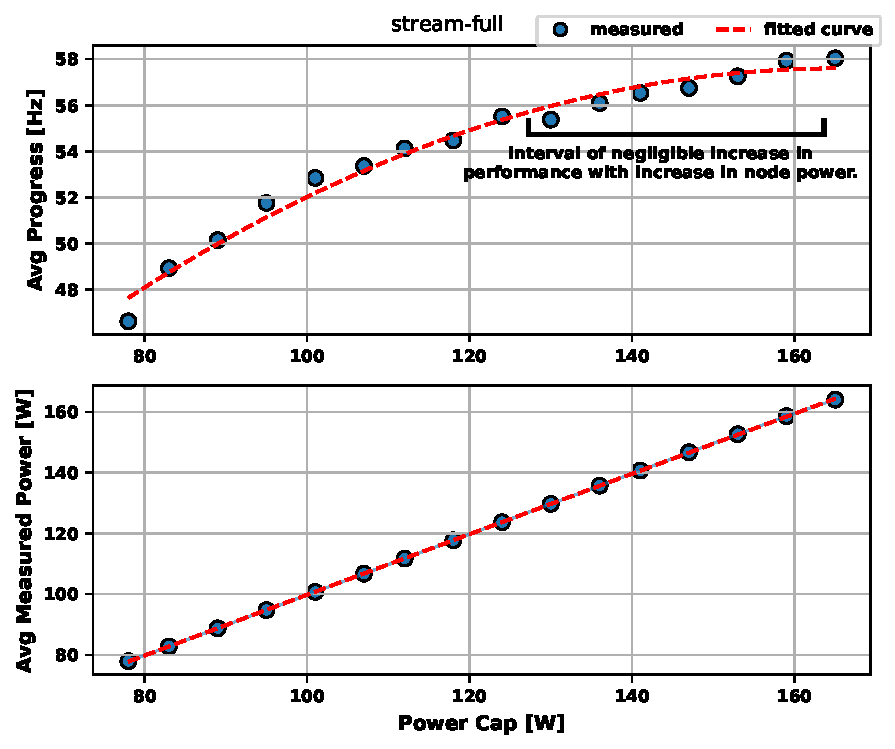
\includegraphics[width=\linewidth]{Figures/ones-stream-full_pcap_analysis.pdf}};

        % Coordinate system: (0,0)=bottom-left, (1,1)=top-right of the image
        % \begin{scope}[x={(img.south east)}, y={(img.north west)}]
        %     % Square-bracket annotation BELOW the plot region
        %     \draw[thick]
        %         (0.55,0.75) -- (0.55,0.72) -- (0.85,0.72) -- (0.85,0.75);
        %     % Annotation text BELOW the bracket
        %     \node[font=\scriptsize, align=center] at (0.67,0.65)
        %         {Interval of negligible increase in \\ performance with increase in node power.};
        % \end{scope}
    \end{tikzpicture}
    \vspace{-0.7cm}
    \caption{{Power vs instantaneous performance (progress) for the \texttt{stream-full} benchmark on an Intel Cascadelake node. Progress, defined in Eq.~\eqref{ch4:eq:progress-calculation}, is a proxy for the instantaneous performance of an application toward its scientific objective.}}
    \label{fig:motivation_fig}
%    \Description{Motivating example}
\end{figure}
% \vspace{-0.3cm}

Figure~\ref{fig:motivation_fig} illustrates this relationship for a memory-bound application, showing instantaneous performance (measured via instrumentation) and corresponding power consumption under varying processor power caps.
A closer examination of the application’s runtime behavior reveals that performance does not scale linearly with increasing power caps. Instead, there exist operating regions in which similar performance levels are achieved at substantially lower power. These regions represent opportunities for energy optimization, which  motivate the need for adaptive power and performance control strategies.
% \todo[color=blue!30]{Need to correct the figures.}
%
% \begin{figure*}
%     \centering
%     \begin{minipage}{0.5\textwidth}
%         \centering
%         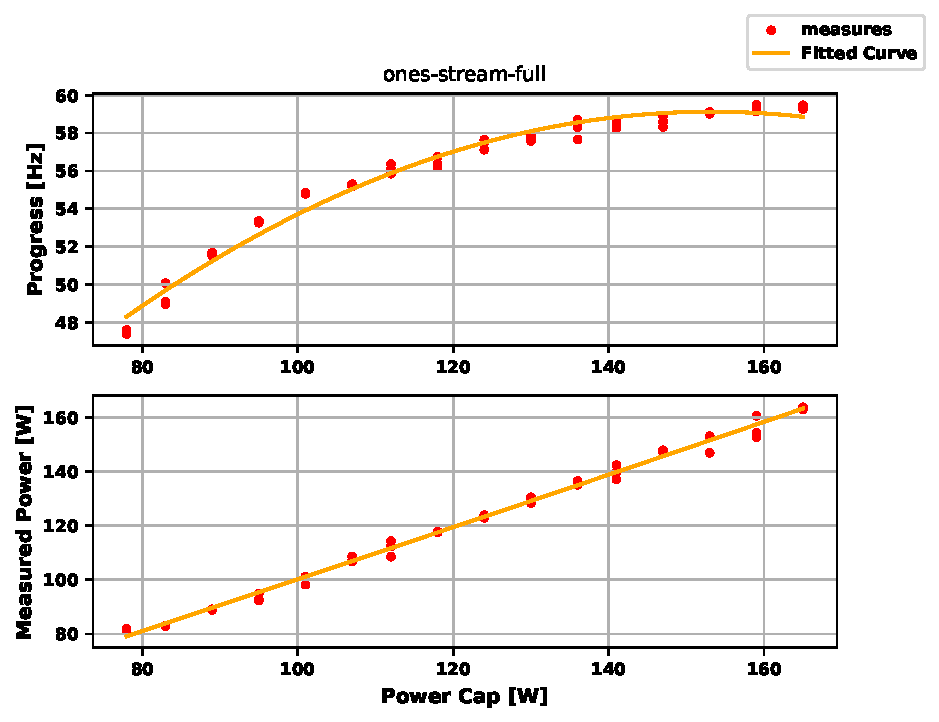
\includegraphics[width=\textwidth]{Figures/static_characteristics_ones-stream-full.pdf} % first figure itself
%         \caption*{\small{STREAM-FULL}}
%         \label{fig:stream-full}
%     \end{minipage}\hfill
%     \begin{minipage}{0.5\textwidth}
%         \centering
%         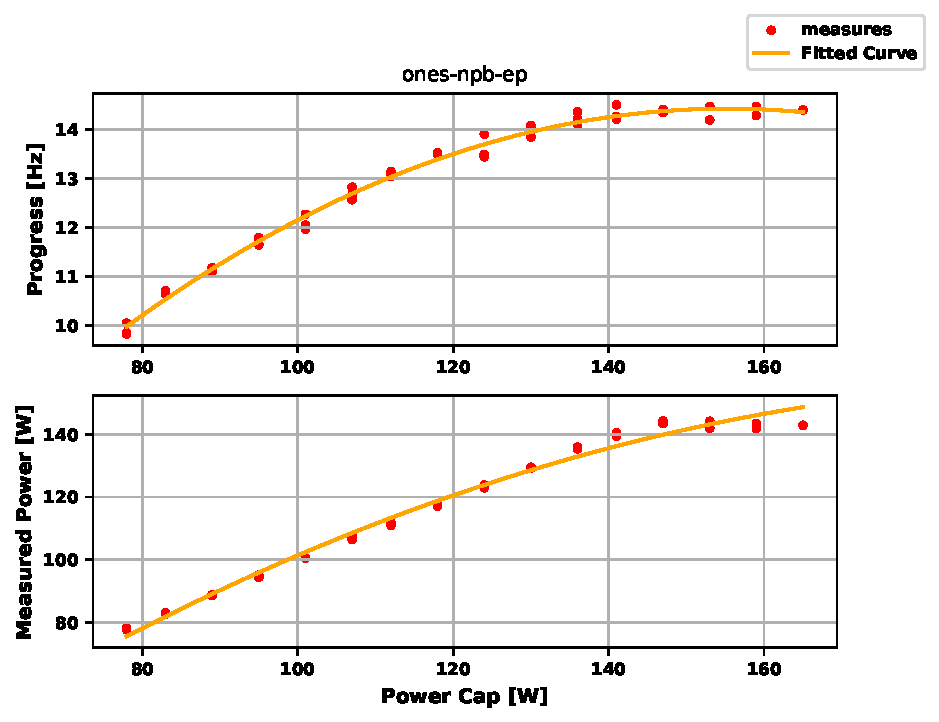
\includegraphics[width=\textwidth]{Figures/static_characteristics_ones-npb-ep.pdf} % first figure itself
%         \caption*{\small{EP}}
%         \label{fig:ep}
%     \end{minipage}
%     \caption{Power vs instantaneuous performance of different applications on an Intel cascadelake processor.}
%     \label{fig:motivation_fig}
%     \Description{Motivating example}
% \end{figure*}
%
%

% \begin{figure}[ht]
% \vspace{-0.5cm}
% {\includegraphics[width=0.5\textwidth,keepaspectratio]{Figures/PCAP_vs_P.pdf}}
% \caption{Relation representing the PCAP vs P in }
% \label{fig:PCAP_vs_P}
% \vspace{-0.5cm}
% \Description{Motivating Example}
% \end{figure}

% With the introduction of modern processors with energy optimization technologies like, Dynamic Voltage and Frequency Scaling (DVFS) \cite{4658633}, Intel's Running Average Power Limit (RAPL) \cite{david2010rapl}, AMD's Thermal Design Power (TDP) Cap \cite{10.1145/3321551} etc. the application oriented power optimization took a turn. Researchers, utilizing the measurement and actuation capabilities available with these technologies, have come up with advanced power control strategies targeted towards energy efficient computing.
% These works that ranges from classical control theory \cite{10.1007/978-3-030-85665-6_21} to machine learning based control \cite{9465707}, are successful in regulating the power at a constant value based on the HPC node and the application it runs. Some of these methods help regulate the power dynamically by observing the changes in performance of the application towards the completion of its scientific goal \cite{10305814}. But all these methods use either a hardware centric or application specific approach, which need changes in parameters with changes in application or architecture. % Decision making based on observing these instantaneous performance needs constant interaction with the HPC node and therefore the algorithms that interact with the node has to be light weight in terms of the memory consumption.

Modern processors with energy optimization capabilities such as dynamic voltage and frequency scaling (DVFS)~\cite{4658633}, Intel's Running Average Power Limit (RAPL)~\cite{david2010rapl} and AMD's thermal design power cap~\cite{10.1145/3321551} have enabled application-oriented power optimization. 
Advanced power control strategies using these technologies range from classical control theory to approaches based on machine learning (ML)~\cite{czarnul2019energy}. These methods can regulate power at a constant value, which is chosen according to hardware and application characteristics. Methods such as Dynamic Energy-Performance Optimizer $DEPO$~\cite{KRZYWANIAK2023396} can even dynamically adjust power by observing changes in application performance. %Despite these efforts, 
Such approaches are, however, either hardware-centric or application-specific: they require recomputing all the parameters whenever the application or hardware changes. To avoid this, we require a solution that is hardware- and application-agnostic.  Therefore, in this paper, we design a power-capping controller that operates without application-specific tuning.


% In contrast, this paper presents the design of an application- and hardware-agnostic controller for energy-efficient computing using reinforcement learning (RL). By application agnostic, we mean that the controller does not rely on the specific nature or characteristics of the application. We  assume only that the applications are iterative in nature, such that an instrumented code segment can be placed within the most frequent iteration to measure the progress of the application toward its scientific objective. Similarly, hardware agnostic implies that the controller does not require any prior knowledge of the underlying system architecture or CPU characteristics for decision-making. 

Reinforcement Learning (RL), which is an online machine learning method, is generally used for control applications, however, like any other ML algorithm, is computationally expensive to train. Therefore, researchers use surrogate models or digital twins of their environments~\cite{10305814} to train RL-agents when interactive learning is not possible. In such cases, the accuracy of the attained control objective depends on the accuracy of the surrogate models used for learning. Unfortunately, in data center or HPC compute clusters, where application and hardware power-to-performance relationship changes across application and hardware architectures, generating a black-box model~\cite{WITT201933} using available datasets is difficult. 

Consequently, we propose an \emph{off-the-node training method} for the RL agent using non-interactive or offline learning~\cite{levine2020offline}, with the data generated from existing arbitrary policies.
Here, the training is offline in nature, i.e., the actual compute node is never queried for evaluating an action during the training phase. Thus, offline RL requires a pre-collected dataset of state transitions, actions and rewards, using which the agent can be trained elsewhere. By training the RL model offline, we reduce the computational burden on the actual compute node and eliminate the need for surrogate models to train the agent.

We evaluate our approach by having it regulate the node-level power cap (PCAP) across multiple compute nodes using 12 benchmark applications. We compare it against several state-of-the-art power management systems~\cite{autoPM,zhangenergy,cerf2021sustaining}. Experimental results show that our scheme outperforms existing methods by reducing average energy consumption by 20\% with an average performance loss of only 7.4\% and a worst-case performance degradation of 14\%. When compared with the manufacturer-provided \textit{on-demand} frequency governor (which dynamically adjusts core frequencies), our method demonstrates superior performance in 
%minimizing the overall objective of 
reducing energy consumption while maintaining performance.

\iffalse 
% Akhilesh, For now I am commenting this out as we are over 10 pages - Andy
The key contributions of this paper are the following:
\begin{itemize}
\iffalse
% This may be too strong a claim. I am toning it down -Andy
\item To the best of our knowledge we demonstrate the first use of offline reinforcement learning for the design of energy efficiency control policies, enabling the design of future policies from existing datasets without access to the system. 
\fi 
% \item We demonstrate a novel use of offline reinforcement learning for the design of energy efficiency control policies, enabling the design of future policies from existing datasets without access to the system. 
\item We design an application and hardware agnostic power-capping controller for HPC systems that integrates lightweight online signals - including application heartbeats and hardware performance counters - to preserve performance while regulating energy use at runtime.
% \textbf{GAIL - These first two items seem really similar. If you demonstrate the first use, it seems it would have to be novel -- unless you describe an unusual use also -- in which case you might want to say what it is}
% \item We present the design of a concrete controller for power capping HPC systems at runtime that combines lightweight application awareness (by monitoring application heartbeats) and hardware performance counters to preserve performance while staying application-agnostic (i.e., without deep performance characterization of each application). 
\item We demonstrate that offline reinforcement learning can be effectively used to learn such energy-efficiency control policies directly from previously collected datasets, enabling policy development without access to the live systems.

\item We validate our control policy on a range of well-established benchmarks characterized by varying arithmetic intensities and behaviors (phases).
\end{itemize}
\fi 

Note that although this work illustrates control design for multisocket CPU-only systems, it is applicable to other resources, and GPUs in particular will be the focus of future work. Further, we posit that a single-node controller can then be integrated into a full-system solution. 
% For example, an overprovisioned system could use system-wide power management to allocate available power to new resources, while using a controller such as ours to regulate the power consumption of allocated nodes.

The remainder of this paper is structured as follows: 
In Section~\ref{ch4:sec:Related} we provide background material and review existing algorithms in power and performance optimization. 
%Section~\ref{ch4:sec:Background} presents the necessary background for this paper, including the RL algorithm, %hardware and software stacks, and packages used in the experiments. 
Section~\ref{ch4:sec:Problem} formulates the problem. 
Section ~\ref{ch4:sec:Methodology} outlines the proposed algorithm and workflow in the context of compute nodes. Section~\ref{sec:setup} presents the experimental setup used in both training and evaluations. 
In Section~\ref{sec:Results} we present the experimental design and implementation, along with the results and analysis. 
Finally, Section ~\ref{ch4:sec:Conclusion} provides  a brief summary, the impact of this work, and future opportunities. 